\chapter{Results}\label{ch:results}


\begin{figure}
 \footnotesize
 \centering
    \begin{subfigure}[]{0.55\textwidth}
              \centering
  		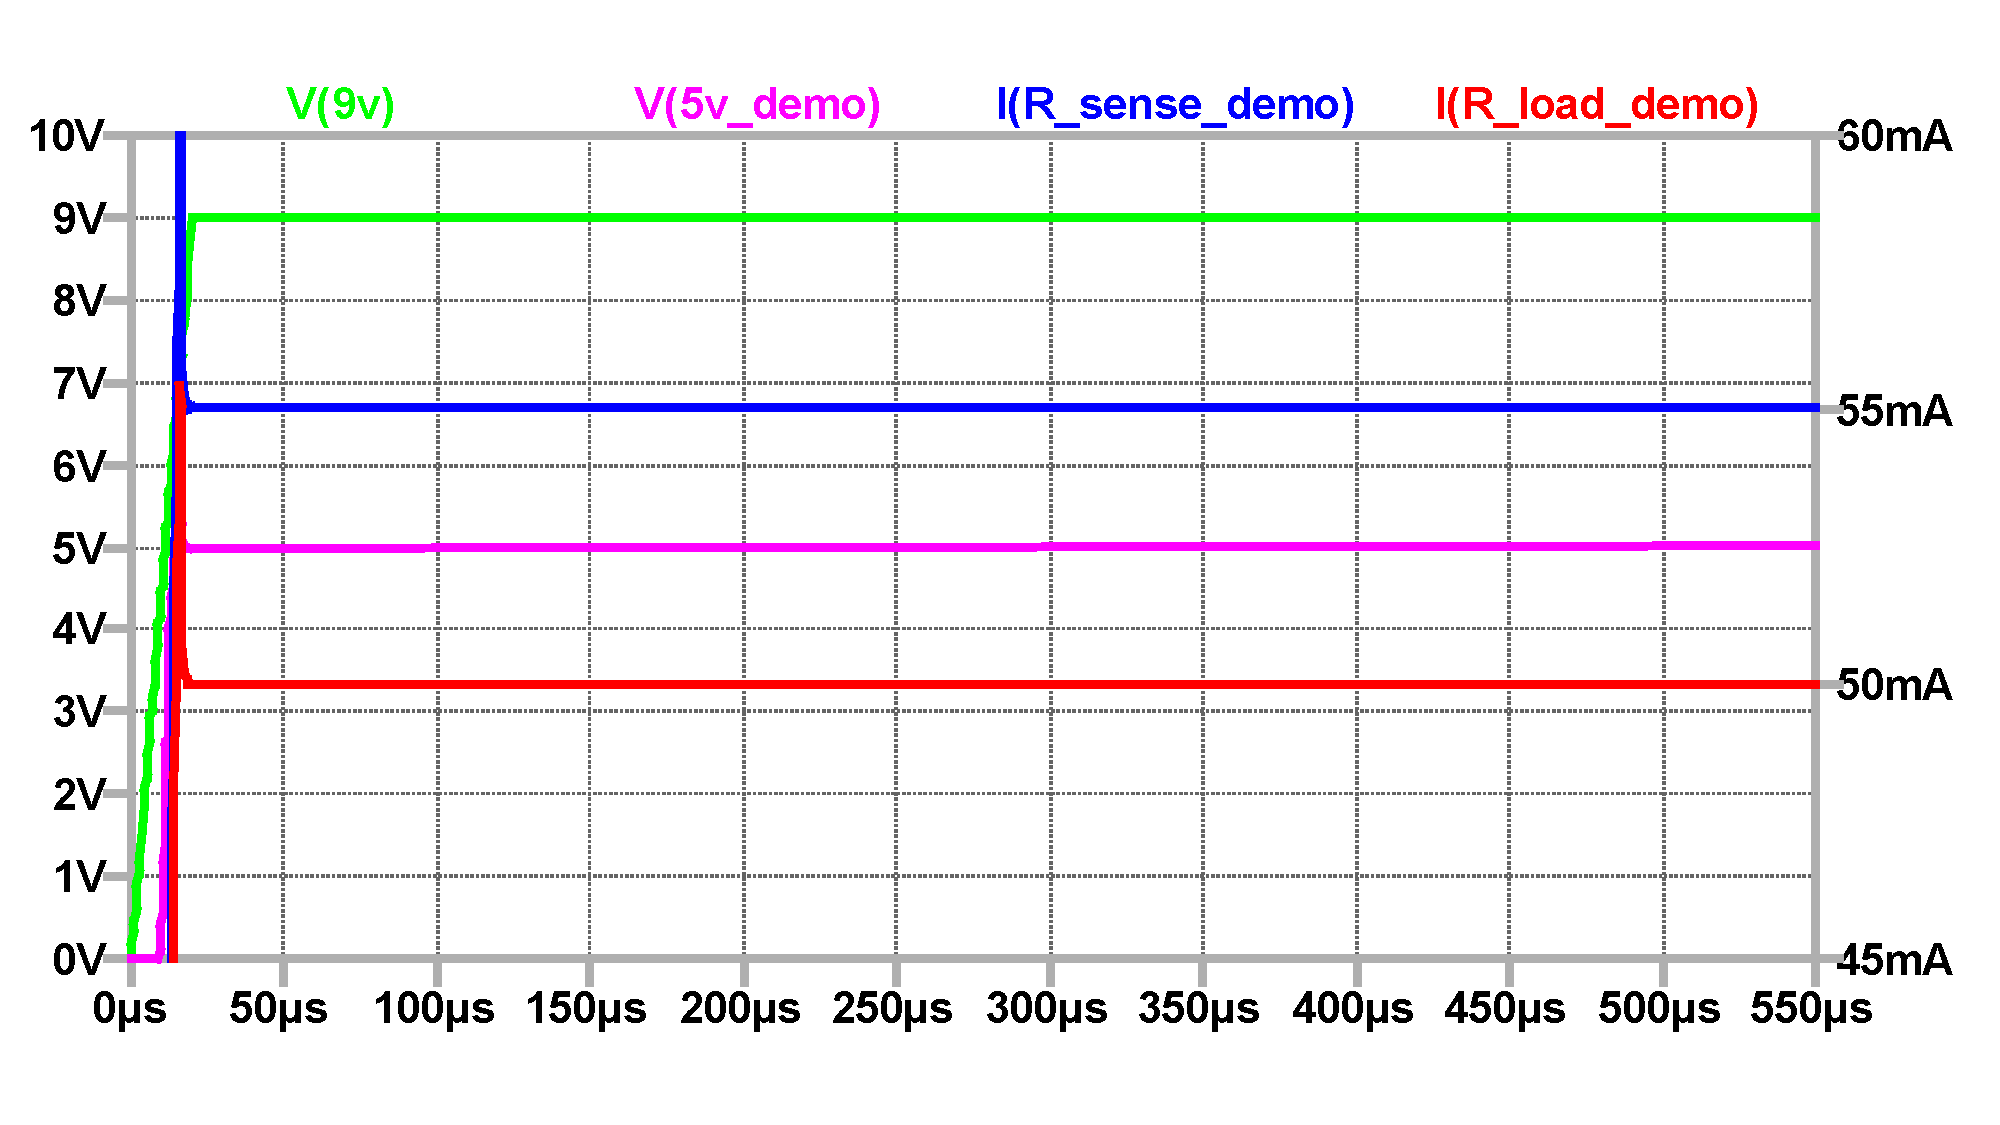
\includegraphics[width=1\linewidth]{./Figures/E344_VoltRegulator.pdf}
		    \caption{} \label{subfig:pwr_simu_rect}
     \end{subfigure}
     \begin{subfigure}[]{0.4\textwidth}
             \centering
  		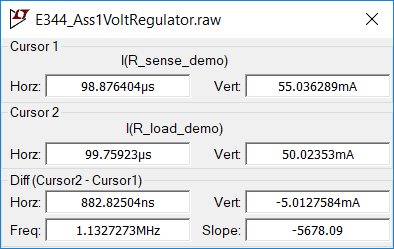
\includegraphics[width=1.0\linewidth]{./Figures/Screengrab2}
		   \caption{ } \label{subfig:pwr_meas_rect}
     \end{subfigure}
    \begin{subfigure}[]{0.55\textwidth}
              \centering
  		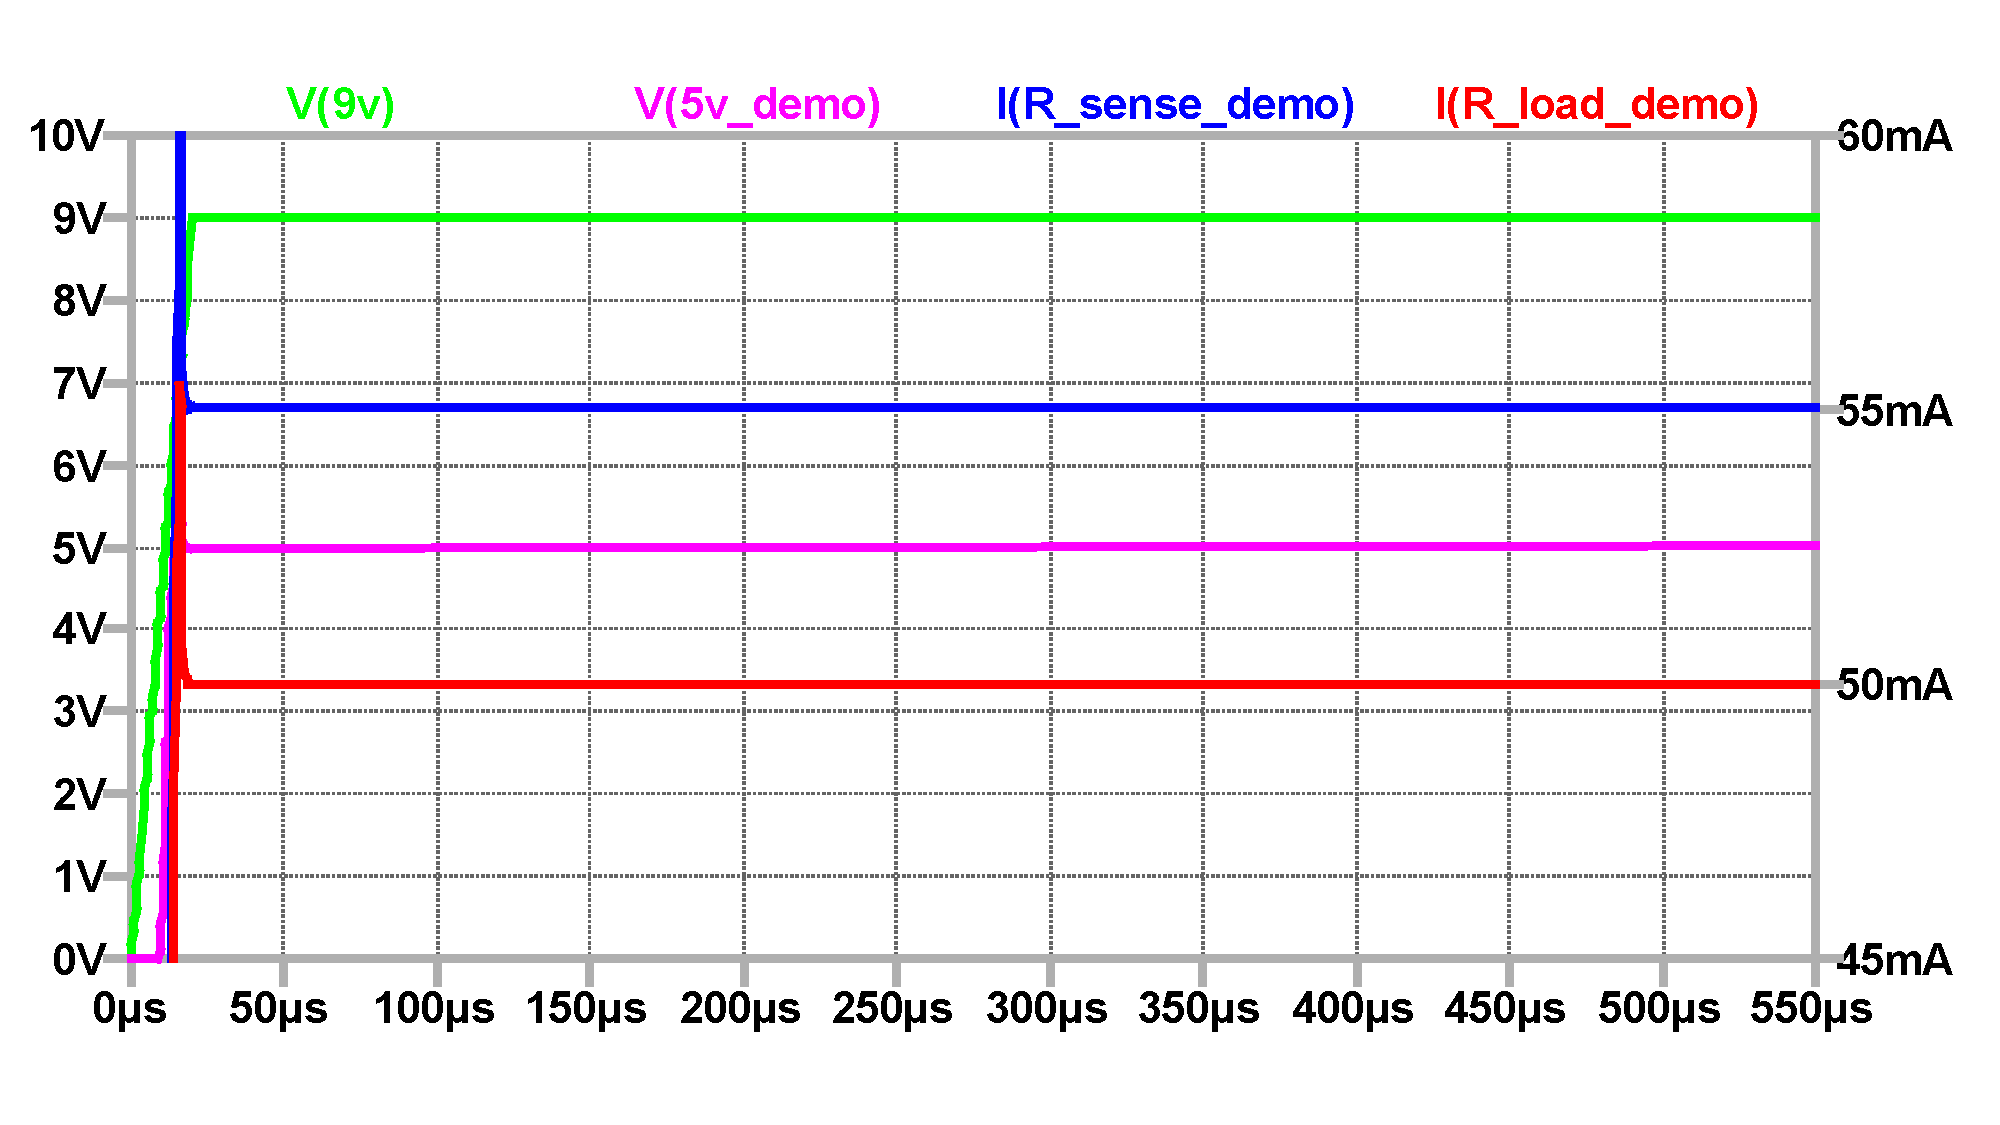
\includegraphics[width=1\linewidth]{./Figures/E344_VoltRegulator.pdf}
		    \caption{} \label{subfig:pwr_simu_rect}
     \end{subfigure}
    \begin{subfigure}[]{0.4\textwidth}
              \centering
  		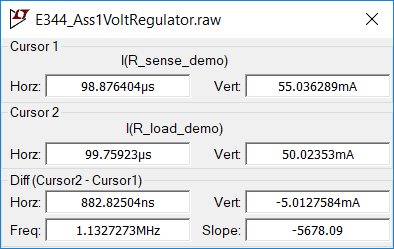
\includegraphics[width=1\linewidth]{./Figures/Screengrab2}
		    \caption{} \label{subfig:pwr_simu_rect}
     \end{subfigure}
   \caption[\textcolor{red}{I am the short caption that appears in the List of Figures list}]{Voltage regulation, comparing the linear and switchmode regulators... (a)  Blah blah. (b)  Blah blah.  (c)  Blah blah. (d) Blah blah.   As far as possible, please put input(s) and output(s) on the same plot rather than on separate plots. Based on the datasheet of XXXX in \cite{WebsiteOpAmp}.}
    \label{fig:simulation_results_box}
 \end{figure}

In this section, you want to demonstrate, by means of referring to simulation results, using the designed circuit, how your circuit behaves as you designed it in Section \ref{sec:current_sensor_design}. Present and report on your simulated results in Figure \ref{fig:simulation_results_box}. Be absolutely sure that the text and information in your report are readable. 

\noindent You can use screengrabs or photos of the oscilloscope, or download the CSVs and plot them as PDFs using Matlab, Excel or similar. 
You can also use tables, example of which are presented in Tables \ref{tab:table1} and \ref{tab:table2}.


\begin{table}[h]
        \centering
        \footnotesize
        \caption{Example of a simple table.}
         \begin{tabular}{c@{\qquad}rrrr}
          \toprule
             & 2017 & 2018 & $\Delta_{Abs}$ & $\Delta_{DiD}$\\
          \midrule
          A & 9,868      & 10,399 & +5 & -11\\
          B & 10,191     & 10,590 & +4 & -12\\
          \bottomrule
        \end{tabular}
     \label{tab:table1}
\end{table}


\begin{table}[h]
         \centering
        \footnotesize
        \caption{Example of another table.}

         \begin{tabular}{c@{\qquad}rrrr}
          \toprule
          \multirow{2}{*}{\raisebox{-\heavyrulewidth}{Schools }} & \multicolumn{2}{c}{Total energy used}& \multicolumn{2}{c}{Change}\\
          \cmidrule{2-5}
            & 2017 & 2018 & $\Delta_{Abs}$ & $\Delta_{DiD}$\\
            & [kWh] & [kWh] & [\%] & [\%] \\
          \midrule
          A & 9,868      & 10,399 & +5 & -11\\
          B & 10,191     & 10,590 & +4 & -12\\
          \bottomrule
        \end{tabular}
     \label{tab:table2}
\end{table}

%**********************************************
\section{Current sensor} \label{sec:current_sense_results}
%**********************************************



